%
% chapter.tex -- Nichtkommutative harmonische Analysis
%
% (c) 2021 Prof Dr Andreas Müller, Hochschule Rapperswil
%
% !TeX spellcheck = de_CH
\chapter{Nichtkommutative harmonische Analysis
\label{buch:chapter:nichtkomm}}
\kopflinks{Nichtkommutative harmonische Analysis}
Die bisher entwickelte Fourier-Theorie funktioniert nur für
abelsche Gruppen.
Das Registrierungsproblem, welches in
Abschnitt~\ref{buch:nichtkomm:section:motivation} vorgestellt wird,
basiert aber auf einer nicht abelschen Gruppe.
Wichtige Komponenten der Problemlösung sind darauf wohldefiniert,
zum Beispiel die Faltung.
Die Gelfand-Transformation verspricht auch, einen Ansatz zur
Vereinfachung des Rechnens mit der Faltung zu geben.
Tatsächlich gibt die allgemeine Theorie der Gelfand-Paare
und der nichtkommutativen harmonischen Analysis einen Ansatz
für Aufteilung des Problems in mehrere Schritte.

%
% 1-motivation.tex
%
% (c) 2023 Prof Dr Andreas Müller
%
\section{Vergleich von Funktionen
\label{buch:einleitung:section:vergleich}}
\kopfrechts{Vergleich von Funktionen}
Harmonische Analysis ist eine Methode, Funktionen in besser
verstandene Komponenten zu zerlegen.
Die Basis dafür ist die Möglichkeit, die ``Ähnlichkeit'' zwischen
Funktionen zu messen.
In diesem Abschnitt soll gezeigt werden, wie diese Idee der
``Ähnlichkeit'' sich natürlich in verschiedenen bekannten
Anwendungen ergibt.
Das Ziel ist, den Weg zum abstrakten Konzept des verallgemeinerten
Skalarproduktes aufzuzeigen.
\index{Skalarprodukt}%

%
% Kovarianz als Mass der Ähnlichkeit von Datenreihen
%
\subsection{Kovarianz als Mass der Ähnlichkeit von Datenreihen}
In der Statistik lernt man, dass Beziehungen zwischen Zufallsvariablen
\index{Zufallsvariable}%
$X$ und $Y$ durch die Kovarianz gemessen werden.
\index{Kovarianz}%
Wir nehmen für die folgende Diskussion der Einfachheit halber an,
dass die Erwartungswerte $E(X)=E(Y)=0$ sind.
\index{Erwartungswert}%
In diesem Fall ist die Kovarianz der Erwartungswert $E(XY)$ des
Produkts der beiden Zufallsvariablen.
Für Stichproben $x_i$ und $y_i$, $i=1,\dots,n$, kann die Kovarianz mit
Hilfe der empirischen Kovarianz
\[
\operatorname{cov}(X,Y)
=
\frac{1}{n}
\sum_{i=1}^n x_iy_i
\]
geschätzt werden.
Abbildung~\ref{buch:einleitung:fig:kovvergleich} zeigt Beispiele
verschiedener Stichproben mit mehr oder weniger grosser
Kovarianz.
Im rechten Teil der Abbildung sind die Paare $(x_i,y_i)$ als
Punktepaare aufgezeichnet.

\begin{figure}
\begin{center}
\begin{tikzpicture}[>=latex,thick]
%\draw (-7,-15.8) rectangle (7,2.7);
\clip (-7,-15.8) rectangle (7,2.7);
\begin{scope}
\node at (0,0) {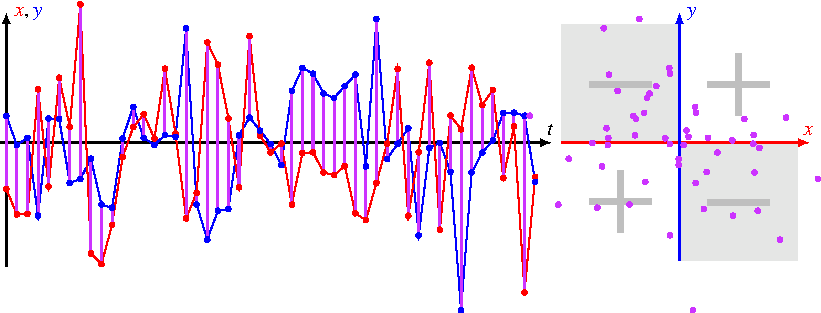
\includegraphics{chapters/000-einleitung/images/randrand.pdf}};
\end{scope}
\begin{scope}[yshift=-4.5cm]
\node at (0,0) {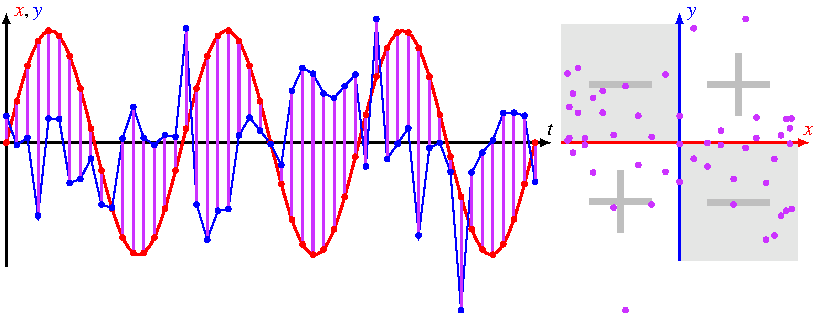
\includegraphics{chapters/000-einleitung/images/sinrand.pdf}};
\end{scope}
\begin{scope}[yshift=-9.0cm]
\node at (0,0) {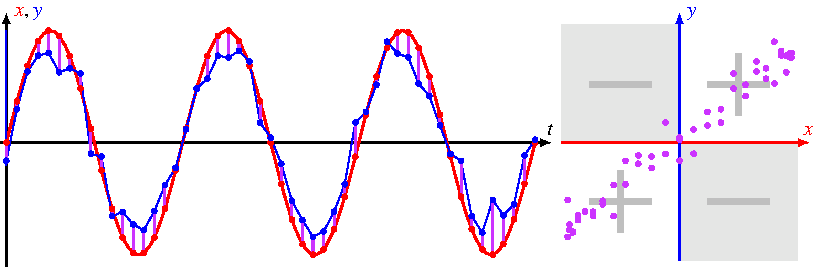
\includegraphics{chapters/000-einleitung/images/sinsin.pdf}};
\end{scope}
\begin{scope}[yshift=-13.5cm]
\node at (0,0) {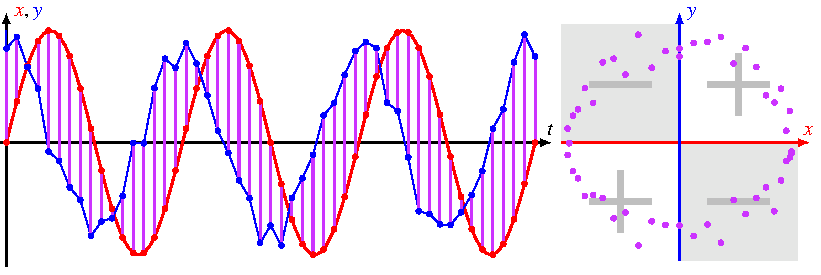
\includegraphics{chapters/000-einleitung/images/sincos.pdf}};
\end{scope}
\end{tikzpicture}
\end{center}
\caption{Stichproben verschiedener Zufallsvariablen mit unterschiedlich
ausgeprägter Kovarianz
\label{buch:einleitung:fig:kovvergleich}}
\end{figure}


Zuoberst in der Abbildung~\ref{buch:einleitung:fig:kovvergleich}
sind zwei ganz zufällige Zahlenreihen dargestellt.
Die Vorzeichen der Produkte $x_iy_i$ sind wild gemischt, die Punkte
verteilen sich gleichmässig über alle vier Quadranten.
Im Mittel heben sich die Beiträge der Produkte $x_iy_i$ weg, die
Kovarianz ist sehr klein.

In der zweiten Graphik ist die rote Zahlenreihe durch eine Sinusfunktion
ersetzt worden.
\index{Sinusfunktion}%
Die $x$-Koordinaten der Punkte sind jetzt nicht mehr zufällig, die
$y$-Koordinaten sind aber immer noch ungeordnet. 
Auch in diesem Fall sind die Punkte gleichmässig über alle Quadranten
verteilt und die Kovarianz ist klein.

In der dritten Graphik sind die blauen Punkte Werte einer
Sinusfunktion, denen kleine zufällige Fehler überlagert sind.
Die Punkte $(x_i,y_i)$ sind jetzt nicht mehr zufällig verteilt,
sie bewegen sich entlang der $45^\circ$-Geraden im ersten
und dritten Quadranten.
Für die meisten Punkte ist das Produkt $x_iy_i$ daher positiv und
die Kovarianz, die Summe dieser Produkte, wird gross.
Die zufällig gestörte blaue Sinusfunktion ist der exakten roten
Sinusfunktion ziemlich ähnlich.

In der letzten Graphik schliesslich werden eine Sinusfunktion und
\index{Cosinusfunktion}%
eine mit zufälligen Abweichungen gestörte Cosinusfunktion miteinenader
verglichen.
Zwar gibt es jetzt einen klaren Zusammenhang, aber die Punkte sind
wieder über alle vier Quadranten verteilt.
Die Kovarianz ist wieder klein.
Tatsächlich ist die gestörte Cosinusfunktion eben nicht ähnlich zu 
einer Sinusfunktion, sondern zu einer Cosinusfunktion.

Die Kovarianz kann also dazu verwendet werden, eine unbekannten
Datenreihe mit verschiedenen Funktionen zu vergleichen und zu
beurteilen, welche am ``ähnlichsten'' ist.

\subsubsection{Zufallsvariablen mit Erwartungswert $\ne  0$}
Für Zufallsvariablen, deren Erwartungswerte nicht verschwinden,
wird die Formel für die Kovarianz etwas komplizierter, sie lautet
\begin{equation}
\operatorname{cov}(X,Y) = E(XY) - E(X)E(Y).
\label{buch:einleitung:eqn:cov}
\end{equation}
Doch dies ändert nichts an der Ähnlichkeit der Kovarianz 
mit einem Skalarprodukt.

Dazu muss man allerdings berücksichtigen, dass zwei Zufallsvariablen
im Vergleich zu den Schwankungen sehr grosse Erwartungswerte haben können.
Dies hat zur Folge, dass $E(XY)$ von den Erwartungswerten dominiert
wird, die Schwankungen spielen nur eine untergeordnete Rolle.

Die Zufallsvariable $X-E(X)$ hat wegen
$E(X-E(X))=E(X)-E(E(X))=E(X)-E(X)=0$ Erwartungswert $0$.
Für Datenreihen $x_i$ und $y_i$ bedeutet dies, dass man
die Koordinaten $x$ und $y$ durch neue Koordinaten ersetzt,
so dass die Punktwolke aus den Punkten $(x_i,y_i)$ den
Nullpunkt des Koordinatensystems als Schwerpunkt hat.
Der Erwartungswert des Produktes von $X-E(X)$ und $Y-E(Y)$
ist dann
\begin{align*}
E(\, (X-E(X))\cdot(Y-E(Y))\, )
&=
E(XY)-E(X\cdot E(Y)) - E(E(X)\cdot Y) + E(E(X)E(Y))
\\
&=
E(XY) - E(X)E(Y)-E(X)E(Y)+E(X)E(Y)
\\
&=
E(XY)-E(X)E(Y),
\end{align*}
dies ist die allgemeine Definition~\eqref{buch:einleitung:eqn:cov}
der Kovarianz.

%
% Das Skalarprodukt in der Vektorgeometrie
%
\subsection{Das Skalarprodukt in der Vektorgeometrie}
Das Skalarprodukt wird in einem rechtwinkligen Koordinatensystem nach der
\index{Skalarprodukt}
Formel
\begin{equation}
\vec{x}\cdot\vec{y} = x_1y_1 + x_2y_2 + x_3y_3 = \sum_{i=1} x_iy_i
\label{buch:einleitung:motiviation:equn:vektorskalar}
\end{equation}
berechnet.
Es verschwindet, wenn die Vektoren $\vec{x}$ und $\vec{y}$ orthogonal
sind, man könnte sagen,
wenn die Vektoren so verschiedene Richtung wie möglich haben.
Die Orthogonalprojektion von $\vec{x}$ auf die Richtung $\vec{y}$,
\index{Orthogonalprojektion}%
auch die Komponente von $\vec{x}$ in der Richtung von $\vec{y}$ genannt,
hat die Länge 
\[
\frac{\vec{x}\cdot\vec{y}}{|\vec{y}|}
=
\vec{x}\cdot \vec{y}^0.
\]
Das Skalarprodukt zweier Vektoren ist nicht grösser als das Produkt
der Vektorlängen.
Die Cauchy-Schwarz-Ungleichung, ausführlich diskutiert in
\index{Cauchy-Schwarz-Ungleichung}%
Abschnitt~\ref{buch:skalarprodukte:section:cauchyschwarz},
zeigt, dass das Skalarprodukt mit dem Produkt der Vektorlängen
genau dann übereinstimmt, wenn die Vektoren die gleiche Richtung
haben, wenn sie also linear abhängig sind.
Die Berechnungsformel~\eqref{buch:einleitung:motiviation:equn:vektorskalar}
deckt sich mit der Formel zur Berechnung der empirischen Kovarianz.

%
% Skalarprodukte von Funktionen
%
\subsection{Skalarprodukte von Funktionen}
Die bisherigen Ausführungen zeigen, dass ein Skalarprodukt von
Vektoren in $\mathbb{R}^n$ als ein Mass für die Ähnlichkeit von Vektoren
dienen kann. 
Die Koordinaten eines Vektors in einer orthogonalen Basis werden
als Skalarprodukte des Vektors mit den Basisvektoren bestimmt.
Die Koordinaten geben an, wie ``ähnlich'' zu den Basisvektoren ein Vektor
ist.
Die Linearkombination der orthonormierten Basisvektoren $b_i$ mit den
Koeffizienten $(x\cdot b_i)$ ergibt wieder den Vektor 
\[
x = \sum_{i=1}^n (b_i\cdot x) \, b_i.
\]
Das Skalarprodukt ist also eine besonders effiziente und natürlich
Methode, einen Vektor in Komponenten parallel zu den Basisvektoren
zu zerlegen und den Vektor auch wieder aus den Basisvektoren zu
synthetisieren.

Diese Idee kann auf sehr viele weitere Situation ausgedehnt werden,
wenn sich das Konzept des Skalarproduktes darauf übertragen lässt.
Aus der linearen Algebra \cite{buch:linalg} weiss man, dass sich
aus den Axiomen eines 
Skalarproduktes und aus einer Basis alles konstruieren lässt, was
man für eine solche Analyse benötigt.
Funktionen bilden bereits einen Vektorraum.
\index{Vektorraum}%
Wenn es also gelingt,
ein Skalarprodukt zu konstruieren, dann kann man damit beginnen,
orthonormierte Basen zur Analyse von Funktionen zu verwenden.

%
% Interessante Basen
%
\subsection{Interessante Basen}
Der Gram-Schmidt-Algorithmus zur Konstruktion einer orthonormierten
\index{Gram-Schmidt-Algorithmus}%
Basis zeigt, dass sich ausgehend von jeder beliebigen linear
unabhängigen Funktionenmenge eine Basis konstruieren lässt.
Zum Beispiel kann man orthonormierte Basen aus Polynomen konstruieren.
Da Polynome sehr leicht zu evaluieren sind, ergeben sich für die
Numerik nützliche Funktionsbasen.
\index{Numerik}%

Meistens haben die Funktionen, die man analysierte möchte, noch
viel mehr Struktur.
Joseph Fourier hat beobachtet, dass periodische Funktionen zu einer
\index{Fourier, Joseph Baptiste}%
besonders erfolgreichen Theorie führen.
Man kann seine Basisfunktion dadurch charakterisieren, dass sie
unter Translation des Arguments invariant sind.
Verlangt man ausserdem Differenzierbarkeit, dann sind die
Fourier-Basisfunktionen Eigenfunktionen des Ableitungsoperators.
\index{Fourier-Basisfunktionen}%
\index{Eigenfunktionen}%
\index{Ableitungsoperator}%

Tatsächlich treten orthogonale Funktionensystem im Zusammenhang
mit partiellen Differentialgleichungen auf ganz natürliche Art auf.
Ist $L$ ein selbstadjungierter Operator, dann sind die Eigenfunktionen
dieses Operators orthogonal.
Die trigonometrischen Funktionen sind zum Beispiel Eigenfunktionen
des Operators der zweiten Ableitung, ausserdem ist die zweite
Ableitung selbstadjungiert im Raum der periodischen Funktionen
mit dem $L^2$-Skalarprodukt.
Der Laplace-Operator hat ähnliche Eigenschaften und führt
auf verallgemeinerte harmonische Analysis für Funktionen auf
einer grossen Zahl von Definitionsgebieten, die auch für
Anwendungen wichtig sind.

Die Fourier-Funktionen haben aber noch weitere wichtige Eigenschaften.
Das Definitionsgebiet hat die Struktur einer Gruppe, was sich zum
\index{Gruppe}%
Beispiel in den Additionstheoremen äussert.
Daraus lässt sich eine weitere Operation konstruieren, die Faltung.
\index{Faltung}%
Es zeigt sich, dass die Verwendung der Fourier-Basis auch dazu führt,
dass die Fourier-Transformation aus einem Faltungsprodukt ein gewöhnliches
\index{Fourier-Transformation}%
Produkt der Fourierkoeffizienten macht.
Auch diese Eigenschaft lässt sich auf eine grosse Zahl weiterer
Gruppen auf interessante Art verallgemeinern.

Es gibt also verschiedene Möglichkeiten, ein Funktionsystem so
zu wählen, dass es einerseits optimal an eine Aufgabenstellung
angepasst ist, andererseits aber eine Analyse mit einem Skalarprodukt
und Synthese ermöglicht.
Das Ziel dieses Seminars ist, diese Möglichkeiten auszuloten
und einige wichtige Anwendungen zu illustrieren.





%
% 2-homogen.tex
%
% (c) 2023 Prof Dr Andreas Müller
%
\section{Homogene Räume
\label{buch:nichtkomm:section:homogeneraeume}}
\kopfrechts{Homogene Räume}
Im vorangegangenen Abschnitt haben wir eine gemeinsame mathematische
Formalisierung für verschiedene Varianten des Registrierungsproblems
gefunden.
In diesem Abschnitt wenden wir uns den Gemeinsamkeiten des 
abstrakten Problems zu und ermitteln die Struktur, die uns später
helfen wird, das Registrierungsproblem auf einheitliche Weise
in einfachere Teilprobleme aufzuteilen.

%
% Stabilisator
%
\subsection{Stabilisator
\label{buch:nichtkomm:homogen:subsection:stabilisator}}
In die grosse Menge der Transformationen des Definitionsbereiches
$X$ lässt sich etwas Ordnung bringen, indem man Fixpunkte dieser
Transformationen sucht.
\index{Fixpunkt}

\begin{definition}[Fixpunkt, Stabilisator]
Wenn die Gruppe $G$ auf dem Raum $X$ operiert und $x\in X$ ist, dann
heisst $x$ ein {\em Fixpunkt} einer Transformation $s\in G$, wenn 
\index{Fixpunkt}%
$s\cdot x = x$ ist.
Die Menge
\[
S_x = \{ s\in G \mid s\cdot x = x \}
\]
aller Transformationen, die $x$ als Fixpunkt haben,
heisst der {\em Stabilisator} von $x$.
\index{Stabilisator}%
\end{definition}

Der Stabilisator eines Punktes $x\in X$ ist immer eine Untergruppe.
Dazu muss man nur überprüfen, ob die Zusammensetzung und die Inverse
von Elementen aus $S_x$ wieder in $S_x$ liegt.
Dies ist aber klar, denn wenn zwei Elemente $g,h\in S_x$ den Punkt $x$
festhalten, dann ist auch $(gh)\cdot x= g\cdot(h\cdot x) = g\cdot x = x$
und analog für die Inverse.

\begin{beispiel}
\label{buch:nichtkomm:homogen:bsp:SO3}
Die Gruppe $\operatorname{SO}(2)\ltimes\mathbb{R}^2$ operiert auf der
Mengen $X=\mathbb{R}^2$.
Nicht jede Transformation hat einen Fixpunkt, zum Beispiel haben reine
Verschiebungen um einen Vektor $v\in\mathbb{R}^2$, $v\ne 0$, keinen
Fixpunkt.
Für eine Transformation $(s,a)\in\operatorname{SO}(2)\ltimes \mathbb{R}^2$
mit $s\ne e$, also eine Transformation mit einer nichttrivialen
Drehkomponente, lässt sich immer ein Fixpunkt durch Lösung der 
Gleichung
\[
sx+a=x
\quad\Rightarrow\quad
x = -(s-e)^{-1}a
\]
ermitteln.
Diese Lösung ist genau dann möglich, wenn $s-e$ invertierbar ist.
Ob eine Matrix invertierbar ist,
kann mit der Determinante entschieden werden.
Die Determinante der Matrix $D_\alpha-I$ ist
\begin{align*}
\det(D_\alpha-I)
&=
(\cos\alpha-1)^2+\sin^2\alpha
\\
&=
\cos^2\alpha-2\cos\alpha +1+\sin^2\alpha
\\
&=
2-2\cos\alpha 
\\
&=
2(1-\cos\alpha).
\end{align*}
Diese verschwindget genau dann, wenn $\alpha$ ein Vielfaches von $2\pi$ ist.
Damit ist gezeigt, dass alle Transformationen mit einer nichttrivialen
Drehkomponente einen Fixpunkt haben.

Der Stabilisator eines Punktes $x\in\mathbb{R}$ besteht aus denjenigen
$(g,a)\in\operatorname{SO}(2)\ltimes \mathbb{R}^2$, für die
\[
(g,a)\cdot x = g\cdot x+a = x
\]
gilt.
Daraus leitet man die Bedingung 
\[
(g-e)\cdot x = -a
\]
ab.
Für jede Drehung $g\in\operatorname{SO}(2)$ gibt es also einen Vektor
$a=-(g-e)$ derart, dass $(g,a)\in\operatorname{SO}(2)\ltimes\mathbb{R}^2$
den Punkt $x$ als Fixpunkt hat.
Die Abbildung $g\mapsto(g,-gx+x)$ ist daher ein Isomorphismus von
$\operatorname{SO}(2)$ auf den Stabilisator
$S_x\subset \operatorname{SO}(2)\ltimes \mathbb{R}^2$.
\end{beispiel}

\begin{beispiel}
Die Gruppe $G=\operatorname{SO}(3)$ operiert auf der Kugeloberfläche $S^2$.
Der Stabilisator eines Punktes $x\in S^2$ auf der Kugeloberfläche besteht
aus allen Drehungen, die die Achse mit Richtung $x$ oder $-x$ fest
lassen.
Die Untergruppe der Drehungen um die Achse ist isomorph zur Gruppe der
zweidimensionalen Drehmatrizen.
Ein Isomorphismus kann wie folgt konstruieren.
Zunächst wählt man zwei Einheitsvektoren $b_1,b_2\in \mathbb{R}^3$ derart,
dass $b_1,b_2$ und $x$ eine orthonormierte Basis bilden.
In dieser Basis können Drehungen $s$ um die Achse $x$ durch Matrizen der Form
\begin{equation}
s
=
\left(
\begin{array}{cc|c}
\cos\alpha & -\sin\alpha & 0 \\
\sin\alpha &  \cos\alpha & 0 \\
\hline
     0     &       0     & 1
\end{array}
\right)
=
\left(
\begin{array}{cc|c}
\multicolumn{2}{c|}{
\multirow{2}{*}{$D_\alpha$}
}&0\\
&&0\\
\hline
0&0&1
\end{array}
\right)
\quad\text{mit}\quad
D_\alpha\in\operatorname{SO}(2)
\label{buch:nichtkomm:homogen:bsp:SO3:op}
\end{equation}
dargestellt werden.
Die Abbildung $D_\alpha\mapsto s$ ist ein Isomorphismus von
$\operatorname{SO}(2)$ auf den Stabilsator $S_x\subset\operatorname{SO}(3)$.
\end{beispiel}

%
% Homogener Raum
%
\subsection{Homogener Raum
\label{buch:nichtkomm:homogen:subsection:homogen}}
Die Definitionsgebiete $X$, die wir im Registrierungsproblem untersuchen,
haben noch eine zusätzliche Eigenschaft.
Für jedes Paar von Punkten $x$ und $y$ in $X$ lässt sich immer mindestens
eine Transformation $g\in G$ finden derart, dass $g\cdot x = y$ ist.
Man sagt, die Gruppe $G$ operiert {\em transitiv} auf $X$.

Typischerweise gibt es nicht nur ein Gruppenelement $g$, welches $x$ in
$y$ transportiert.
Ist $s\in S_x$, dann ist auch $gsx=gx=y$ und für $t\in S_y$ ist
auch $tgx=ty=y$.

\begin{satz}
Falls $gx=hx=x$, dann gibt es eine Element $s\in S_x$ derart, dass
$gs=h$.
\end{satz}

\begin{proof}[Beweis]
Aus $gx=hx$ folgt $x=g^{-1}hx$, also $s=g^{-1}h\in S_x$.
Ausserdem ist $gs=gg^{-1}h=h$, wie verlangt.
\end{proof}

\begin{satz}[Isomorphie der Stabilisatoren]
Wenn die Gruppe $G$ transitiv auf dem Raum $X$ operiert und $x,y\in X$
zwei Punkte in $X$ sind, dann sind die Stabilisatoren $S_x$ und $S_y$
isomorph.
Ist $gx=y$ dann ist die Abbildung
\[
c_g\colon
S_y\to S_x: h\mapsto ghg^{-1}
\]
ein Isomorphismus der Stabilisatoren.
\end{satz}

\begin{proof}[Beweis]
Zunächst können wir leicht nachrechnen, dass $c_g$ ein Homomorphismus ist,
denn
\[
c_g(hk)
=
ghkg^{-1}
=
gh(g^{-1}g)kg^{-1}
=
(ghg^{-1})gkg^{-1})
=
c_g(h)c_g(k).
\]
Wir müssen überprüfen, dass $c_g(s)\in S_y$ ist, wenn $s\in S_x$ ist.
Dazu rechnen wir nach, dass
\begin{equation}
c_g(s)y = gsg^{-1} y = gsx=gx=y
\quad\Rightarrow\quad
c_g(s)\in S_x.
\label{buch:nichtkomm:homogen:eqn:cgimage}
\end{equation}
Der Homomorphismus $c_g$ ist aber auch umkehrbar, denn es gilt
\[
c_gc_{g^{-1}}(h)
=
g(g^{-1}hg)g^{-1}h
=
h
\quad\Rightarrow\quad
c_gc_{g^{-1}}=\operatorname{id}.
\]
Aus \eqref{buch:nichtkomm:homogen:eqn:cgimage} folgt jetzt, dass
$c_{g^{-1}}\colon S_y\to S_x$.
Somit ist $c_g$ ein Isomorphismus.
\end{proof}

Der Satz besagt also, dass in jedem Punkt des Raumes $X$ der gleiche
Stabilisator gefunden wird.
Mit den  Mitteln der Gruppentheorie von $G$ lassen sich zwei Punkte 
in $X$ nicht unterscheiden.
Diese spezielle Situation hat einen Namen.

\begin{definition}[homogener Raum]
Ein Raum $X$, auf dem eine Gruppe $G$ transitiv wirkt, heisst
{\em homogen}, wenn der Stabilisator in jedem Punkt von $x$ gleich ist.
\index{homogen}%
\index{homogener Raum}%
\end{definition}

Da die Gruppe $G$ transitiv auf $X$ wirkt, kann man die Punkte $y$ von 
$X$ auch durch die Transformationen bechreiben, die einen gewählten
Punkte $x$ in $y$ überführen.
Die Tatsache, dass der Stabilisator in jedem Punkt isomorph ist, 
bedeutet, dass der Raum in jedem Punkt ``gleich aussieht'', er hat
hat dort die gleiche Symmetriegruppe.
Ein homogener Raum ist also ein Raum mit einer Gruppenoperation derart,
dass alle Punkte isomorphe Symmetrieuntergruppen haben.

\begin{beispiel}
Sei $x$ der Nordpol der zweidimensionalen Kugeloberfläche $S^2$.
Ist $y\in S^2$ ein weiterer Punkt, gibt es eine Drehung um die Achse,
die durch das Vektorprodukt
$x\times y$ gegeben ist.
Sie transportiert den Nordpol in den Punkt $y$ transportiert.
Alle anderen Drehungen, die den Nordpol in den Punkt $y$ überführen,
bestehen aus einer Drehung um die Nord-Süd-Achse gefolgt von der
genannten Drehung um $x\times y$.
\end{beispiel}

%
% Der Quotientenraum
%
\subsection{Der Quotientenraum $G/K$
\label{buch:nichtkomm:homogen:subsection:quotientgk}}
Sie $G$ eine topologische Gruppe und $K$ eine Untergruppe, die auf $G$
von rechts wirkt.
Zu jedem Element $g\in G$ ist $gK$ die Menge aller Gruppenelemente, 
die mit Hilfe der Rechtsoperation mit einem Element von $K$ erreicht
werden können.
$gK$ heisst auch der {\em Rechtsorbit} oder einfach {\em Orbit} von $g$
bezüglich der Operation von $K$ auf $G$ von rechts.

\begin{definition}[Orbitraum]
Die Menge 
\[
G/K
=
\{ gK \mid g\in G\}
\]
heisst der {\em Orbitraum} der Wirkung von $K$ auf $G$.
\end{definition}

%
% Grenzwertbegriff auf G/K
%
\subsubsection{Grenzwertbegriff auf $G/K$}
Es ist nicht selbstverständlich, dass der Orbitraum
mit einem brauchbaren Grenzwertbegriff ausgestattet
werden kann.

\begin{beispiel}
Die Gruppe $\mathbb{Z}\subset\mathbb{R}$ ist abelsch, der Orbit einer
Zahl $x\in\mathbb{R}$ besteht aus allen Zahlen, die den gleichen
Nachkommateil haben wie $x$.
Sie können dargestellt werden durch die Zahlen im halboffenene
Intervall $[0,1)$.
Die Folge $x_n = 1-1/n\in [0,1)$ konvergiert gegen $1$, was im gleichen
Orbit wie $0$ liegt.
Als topologischer Raum muss man den Orbitraum also mit den
Punkten einer Kreislinie, die man zum Beispiel durch die
Parametrisierung $\mathbb{R}\to S^1:x\mapsto e^{2\pi ix}$ 
beschreiben kann, die $\mathbb{R}$ surjektiv auf $S^1$ abbildet.
\end{beispiel}

Der Orbitraum des vorangegangenen Beispiels der reellen Zahlen
modulo $\mathbb{Z}$ ist sogar eine Gruppe.

\begin{beispiel}
Sei $G=\mathbb{R}/\mathbb{Z}$,
$\alpha\in [0,1)$ eine beliebige Zahl und $K=\alpha\mathbb{Z}$
die Menge aller Vielfachen von $\alpha$ in $G$.
$K$ ist eine Untergruppe von $G$.
Die Menge $K$ ist abzählbar unendlich aber $G$ ist überabzählbar,
der Orbitraum muss also überabzählbar unendlich sein.

Ist $\alpha\in\mathbb{Q}$, dann sei $\alpha=p/q$ die Darstellung
von $\alpha$ als gekürzter Bruch.
Da $q\alpha=p$ ganzzahlig ist, gilt in $G$, dass $q\alpha=0$ ist.
Da der Bruch gekürzt ist, ist $q$ die kleinste Zahl mit dieser
Eigenschaft.
Die Untergruppe $K$ ist in diesem Fall die $q$-elementige endliche
Untergruppe
\[
K = \biggl\{ \frac1qk \;\bigg|\; k=0,\dots,q-1 \biggr\}
\]
von $G$.
Die Orbits von $G/K$ bestehen aus den Elementen, die gleich grossen
Unterschied zum nächstkleineren Element von $K$ aufweisen.
Die Abbildung $q\colon G \to G: x\mapsto qx$ bildet die ganze
Untergruppe $K$ auf $0$ ab und das Intervall $[0,\frac1q)$ auf
$[0,1)$, was zeigt, dass $G/K$ wie $G$ selbst eine Kreislinie ist.

Ist $\alpha\not\in \mathbb{Q}$, dann sind die ganzzahligen Vielfachen
von $\mathbb{Q}$ alle verschieden und bilden eine Untergruppe von $G$,
die jedem Element von $G$ beliebig nahe kommt.
Der Orbitraum ist zwar immer noch eine überabzählbar unendliche
Menge, aber es ist nicht möglich, einen sinnvollen Grenzwertbegriff
zu konstruieren.
Die Folge der Zahlen $x_k=k\alpha$ kommt zwei beliebigen Elementen
von $G$ immer wieder beliebig nahe, sie müssten daher auch in $G/K$
als beliebig nahe beeinander betrachtet werden.
\end{beispiel}

Der Unterschied zwischen den Fällen $\alpha\in\mathbb{Q}$ und
$\alpha\not\in\mathbb{Q}$ äussert sich in der Tatsache, dass
die von $\alpha$ erzeugte Teilmenge $\alpha\mathbb{Z}\subset G$ 
im ersten Fall eine abgeschlossene Teilmenge von $G$ ist,
im zweiten Fall aber nicht.
Dies wird auch durch das folgende Beispiel illustriert.

\begin{beispiel}
Sei $G=\mathbb{R}^2/\mathbb{Z}^2 = (\mathbb{R}/\mathbb{Z})^2$,
also Paare von Elementen der additiven abelsche Gruppe der reellen
Zahlen modulo $\mathbb{Z}$ wie im vorangegangenen Beispiel.
Sei ausserdem $K=\{(k,\alpha k)\mid k\in\mathbb{R}\}\subset G$
die Untergruppe, die durch die Konstante $\alpha$ definiert wird.
Je nachdem ob $\alpha$ rational oder irrational ist, ist die Menge der
Orbits völlig verschieden.

Ist $\alpha\in\mathbb{Q}$, dann gibt es eine Darstellung $\alpha=p/q$
als gekürzter Bruch.
Dies bedeutet, dass $K$ als Teilmenge von $[0,1)$ aus $q$ parallelen
Strecken besteht.
Die Orbits von $K$ bestehen aus den Punkten von $[0,1)$, die gleich weit
vom nächsten ``darunterliegenden'' Geradenstück entfernt sind.
Der Orbitraum ist also wieder $\mathbb{R}/\mathbb{Z}$.

Ist $\alpha\not\in\mathbb{Q}$, dann kommt $K$ jedem Punkt von $G$ beliebig
nahe, $K$ ist also nicht abgeschlossen in $G$ und wie im vorangegangenen
Beispiel ist lässt sich kein nützlicher Grenwertbegriff definieren.
\end{beispiel}

Wir schränken daher im folgenden die Verwendung des Begriffs des
Orbitraums $G/K$ auf Fälle ein, in denen die Untergruppe $K$ eine
abgeschlossene Untergruppe von $G$ ist.
Diese Bedingung ist insbesondere dann immer erfüllt, wenn $K$ eine
kompakte Untergruppe ist.

%
% Linksorbits
%
\subsubsection{Linksorbits}
Alle Begriffe, die im vorangegangenen Abschnitt für die Rechtsoperation
der Untergruppe $K$ auf $G$ entwickelt wurden, lassen sich genauso
auch für die Linksoperation von $K$ auf $G$ entwicklen.
Der zugehörige {\em Links-Orbitraum} ist die Menge
\[
K\backslash G
=
\{ Kg \mid g\in G \},
\]
wie im Falle von $G/K$ kann sie nur dann mit einem nützlichen
Grenzwertbegriff versehen werden, wenn $K$ abgeschlossen ist.

\begin{beispiel}
\label{buch:nichtkomm:homogen:bsp:so2r2}
\begin{figure}
\centering
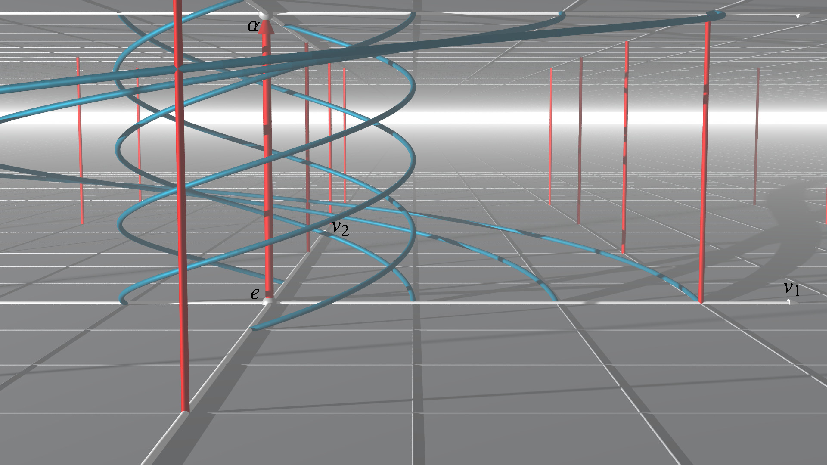
\includegraphics{chapters/070-nichtkomm/images/so2r2.pdf}
\caption{Visualisierung der Gruppe $\operatorname{SO}(2)\ltimes \mathbb{R}^2$
als dreidimensionale Mannigfaltigkeit.
Die Ebene aufgespannt von den Vektoren $v_1$ und $v_2$ ist der Faktor
$\mathbb{R}^2$.
Die Drehungen in $\operatorname{SO}(2)$ werden parametrisiert durch
die auf der vertikalen Achse abgetragenen Drehwinkel $\alpha$, die 
aus dem Intervall $[0,2\pi)$.
Die roten und blauen Kurven zeigen die Rechts- bzw.~Linksorbits
(siehe Beispiel~\ref{buch:nichtkomm:homogen:bsp:so2r2}).
\label{buch:nichtkomm:homogen:fig:so2r2}}
\end{figure}
Die Gruppe $G=\operatorname{SO}(2)\ltimes \mathbb{R}^2$ ist in 
Abbildung~\ref{buch:nichtkomm:homogen:fig:so2r2} visualisiert.
Die horizontalen Ebenen mit Basisvektoren $v_1$ und $v_2$ 
entsprechen dem Faktor $\mathbb{R}^2$.
Auf der vertikalen Achse ist der Drehwinkel $\alpha$ einer Drehung
im Faktor $\operatorname{SO}(2)$ des semidirekten Produktes abgetragen.

Die Elemente $s\subset \operatorname{SO}(2)=K$ werden als Paare
$(s,0)\in \operatorname{SO}(2)\ltimes\mathbb{R}^2$ eingebettet.
Die Rechtsorbits der Operation von $\operatorname{SO}(2)$ auf
$\operatorname{SO}\ltimes \mathbb{R}^2$ sind daher die roten vertikalen
Linien in der Abbildung.
Der Orbitraum
$G/K
=
\operatorname{SO}(2)\ltimes\mathbb{R}^2/\operatorname{SO}(2)$
kann daher mit der Ebene identifiziert werden.

Die Multiplikation mit einer Drehung $s$ mit Drehwinkel $\alpha$ von
Links fügt der ersten Komponente eines Elements $(t,v)$ von
$\operatorname{SO}(2)\ltimes\mathbb{R}^2$ den Drehwinkel hinzu, 
verschiebt den zugehörigen Punkt in
Abbildung~\ref{buch:nichtkomm:homogen:fig:so2r2}
Punkt um $\alpha$ nach oben.
Auf der Vektorkomponente $v$ wirkt $s$ dagegen als Drehung.
So entstehen die blauen Spiralen in
Abbildung~\ref{buch:nichtkomm:homogen:fig:so2r2}
als
Linksorbits der Wirkung von $\operatorname{SO}(2)$ auf $G$.
\end{beispiel}

%
%  Homogene Räume als Quotientenräume
%
\subsubsection{Homogene Räume als Quotientenräume}
Wir betrachten einen homogenen Raum $X$, auf dem die Gruppe $G$
transitiv wirkt.
Sei $x\in X$ ein Punkt von $X$ und $S_x$ der Stabilisator des
Punktes $x$.
Wir betrachten die Abbildung
\[
f
\colon
G\to X
:
g \mapsto x.
\]
Sie ist surjektiv, weil die Gruppe transitiv auf $X$ wirkt und
daher jeden beliebigen Punkt von $x$ aus erreichen kann.

Die Untergruppe $S_x\in G$ operiert durch Rechtsoperation auf $G$.
Wegen $sx=x$ für $s\in S_x$ gilt für die Elemente des Orbits
$gS_x$, dass sie den Punkt $x$ alle auf den gleichen Punkt
\(
gsx = gx
\)
abbilden.
Die Abbildung $f$ bildet daher $S_x$-Orbits bijektiv auf die
Punkte von $X$ ab.

\begin{satz}
\label{buch:nichtkomm:homogen:satz:homorbitraum}
Ist $X$ ein homogener Raum, auf dem die Gruppe $G$ durch Linksoperation
transitiv wirkt, und ist $S_x$ der Stabilisator eines Punktes $x$, dann
ist die Abbildung
\[
f
\colon
G/S_x \to  X
:
gS_x \mapsto gx
\]
ein Homöomorphismus.
\end{satz}

Der Satz zeigt, dass es gar nicht nötig ist, abstrakte homogene Räume
zu betrachten, da solche immer als Orbitraum einer Gruppenoperation 
konstruiert werden können.

\begin{beispiel}
\label{buch:nichtkomm:homogen:bsp:SO3/SO2}
Im Beispiel~\ref{buch:nichtkomm:homogen:bsp:SO3} wurde gezeigt,
die Gruppe $\operatorname{SO}(3)$ transitiv auf der Kugeloberfläche
$S^2$ wirkt und dass der Stabilisator des Nordpols der Kugel
eine Untergruppe $\operatorname{SO}(2)\subset\operatorname{SO}(3)$ ist.
Aus Satz~\ref{buch:nichtkomm:homogen:satz:homorbitraum} folgt nun,
dass die Kugel $S^2\cong \operatorname{SO}(3)/\operatorname{SO}(2)$
ist.
Orbits bestehen aus den orthogonalen Matrizen, die sich nur durch
Multiplikation mit einer Matrix $s$ wie in 
\eqref{buch:nichtkomm:homogen:bsp:SO3:op}
unterschieden.
Ein Matrix in $\operatorname{SO}(3)$ besteht aus orthonormierten 
Zeilen, von denen die letzte bei Multiplikation mit $s$ fest bleibt.
Die ersten zwei Zeilen sind orthogonal auf der dritten und werden durch
$s$ ineinander übergeführt.
Die Orbits bestehen also aus den orthogonalen Matrizen mit der gleichen
letzten Zeile.
\end{beispiel}

%
% Gruppenoperation auf $G/K$
%
\subsubsection{Gruppenoperation auf $G/K$
\label{buch:nichtkomm:homogen:subsection:opaufgk}}
Der Satz~\ref{buch:nichtkomm:homogen:satz:homorbitraum} zeigt, dass
ein homogener Raum $X$ als topologischer Raum immer mit dem Orbitraum
$G/S_x$ identifiziert werden kann, wobei $S_x\subset G$ ein abgeschlossene
Untergruppe ist.
Aber auch die Gruppenoperation der Gruppe $G$ auf $G/S_x$ von links
stimmt mit der Operation auf $X$ überein.

\begin{beispiel}
In Beispiel~\ref{buch:nichtkomm:homogen:bsp:SO3/SO2} wurde darauf
hingewiesen, dass die Kugeloberfläche $S^2$ der homogene Raum
$\operatorname{SO}(3)/\operatorname{SO}(2)$ ist.
Die Orbits bestehen aus orthogonalen Matrizen mit der gleichen letzten
Zeile.
Die Multiplikation mit einer Matrix $s$ wie in 
\eqref{buch:nichtkomm:homogen:bsp:SO3:op}
ist eine Drehung der Kugel um die vertikale Achse.
\end{beispiel}

%
% Registrierungsproblem
%
\subsubsection{Registrierungsproblem für ein Paar von Gruppen}
Das Registrierungsproblem für Bilder in einer Ebene besteht
darin, ein Element von $G=\operatorname{SO}(2)\ltimes \mathbb{R}^2$
zu finden, welches zwei Funktionen in der Ebene $X=\mathbb{R}^2$
zur Deckung bringt.
Die Gruppe wirkt aber transitiv auf $X$ mit Stabilisator
$\operatorname{SO}(2)$, also ist $X$ ein homogener Raum.
Wegen $X=\operatorname{SO}(2)\ltimes\mathbb{R}^2/\operatorname{SO}(2)$
wird das Registrierungsproblem vollständig durch die Angabe
der Gruppe $G=\operatorname{SO}(2)\ltimes \mathbb{R}^2$ und
die abgeschlossene Untergruppe $\operatorname{SO}(2)$ festlegt.

Beim Registrierungsproblem für Funktionen auf der Kugeloberfläche
$S^2$ wurde ähnlich festgestellt, dass die Gruppe $\operatorname{SO}(3)$
transitiv darauf wirkt mit Stabilisator $\operatorname{SO}(2)$ und
dass $S^2\cong \operatorname{SO}(3)/\operatorname{SO}(2)$.
Auch hier spezifiziert das Paar der Gruppen $G=\operatorname{SO}(3)$
und $K=\operatorname{SO}(2)$ das Registrierungsproblem vollständig.





%%
% 1-beispiele.tex
%
% (c) 2023 Prof Dr Andreas Müller, OST Ostschweizer Fachhochschule
%
\section{Beispiele
\label{buch:nichtkomm:section:beispiele}}
\kopfrechts{Beispiele}


%%
% 2-unimodular.tex
%
% (c) 2022 Prof Dr Andreas Müller, OST Ostschweizer Fachhochschule
%
\section{Unimodularität
\label{buch:nichtkomm:section:unimodular}}
\kopfrechts{Unimodularität}

%%
% 3-mittelung.tex
%
% (c) 2022 Prof Dr Andreas Müller, OST Ostschweizer Fachhochschule
%
\section{Mittelungsoperation
\label{buch:nichtkomm:section:mittelung}}
\kopfrechts{Mittelungsoperation}

%%
% 4-gelfand.tex
%
% (c) 2022 Prof Dr Andreas Müller
%
\section{Charaktere und Gelfand-Transformation
\label{buch:gruppen:section:gelfand}}
\kopfrechts{Charaktere und Gelfand-Transformation}
In diesem Abschnitt suchen wir nach weiteren Möglichkeiten, einen
Zusammenhang zwischen der Algebra der Funktionen auf $G$ mit der Faltung
als Multiplikationsoperation und der Gruppe zu rekonstruieren.

%
% Charaktere der Faltungsalgebra
%
\subsection{Charaktere der Faltungsalgebra}
Die Faltung ist eine ziemlich komplizierte Operation.
Der Vektorraum der Funktionen auf $G$ ist ein unendlichdimensionaler
Vektorraum.
Die Unübersichtlichkeit der Faltung und die Dimension kann etwas
vorborgen werden, indem man komplexwertige Abbildungen untersucht,
die möglichst viel der Struktur erhalten.

\begin{definition}
Ein Vektorraum $A$ heisst {\em Algebra}, wenn aus auf $A$ eine bilineare
und assoziative Multiplikation $A\times A\to A$.
Wenn auf dem Vektorraunm $A$ ausserdem eine Norm definiert ist, dann
heisst $A$ eine normierte Algebra, wenn die Multiplikation die
Ungleichung
\[
\| xy \| \le \|x\|\cdot \|y\|\quad\text{für alle $x,y\in A$}.
\]
\end{definition}

\begin{definition}
Sei $A$ eine normierte Algebra.
Ein Charakter $\chi$ ist eine lineare Abbildung $\chi\colon A\to\mathbb{C}$,
die auch ein stetiger Algebrahomomorphismus ist, d.~h.~es gilt
$\chi(xy)=\chi(x)\chi(y)$.
\end{definition}

Als Beispiel betrachten wir den Vektorraum $C([a,b])$ der stetigen Funktionen
auf dem Intervall $[a,b]$ mit der Supremum Norm.
$C([a,b])$ ist aber auch eine Algebra, da Funktionen punktweise
multipliziert werden können.
Wenn $f,g\in C([a,b])$ zwei stetige Funktionen sind, dann ist
$fg\colon [a,b]\to\mathbb{C}:x\mapsto f(x)g(x)$ ein bilineares und
stetigs Produkt.
Für jeden Punkt $x\in[a,b]$ ist
\[
\chi_x
\colon
C([a,b] \to \mathbb{C}
:
f\mapsto f(x)
\]
eine stetige lineare Abbildung.
Sie ist aber auch ein Algebrahomomorphismus.
Dazu muss man nachrechnen, dass $\chi_x(fg)=\chi_x(f)\chi_y(f)$ ist.
Einsetzen der Definition von $\chi_x$ ergibt
\[
\chi_x(fg)
=
(fg)(x)
=
f(x)g(x)
=
\chi_x(f)\chi_x(g).
\]
Es gibt also zu jedem Punkt des Definitionsbereichs einen Charakter
der Algebra $C([a,b])$.

Man kann zeigen, dass die Homomorphismen von der Form $\chi_x$ 
die einzigen Homomorphismen $A\to\mathbb{C}$ sind.
Dies bedeutet, dass sich der Definitionsbereich der Algebra der
stetigen Funktionen vollständig aus der Algebra rekonstruiert werden 
kann.
Der Unterschied ist aber, dass die $[a,b]$ einfach nur eine Menge ist,
während $C([a,b])$ eine reichhaltige Algebrastruktur hat.

\begin{definition}
\label{buch:gruppen:gelfand:def:spektrum}
Ist $A$ eine Algebra, dann heisst die Menge
\[
\mathrm{X}(A)
=
\operatorname{Hom}(A,\mathbb{C})
\]
der Algebrahomomorphismen von $A$ nach $\mathbb{C}$ heisst das
{\em Spektrum} der Algebra $A$.
\end{definition}

Das Spektrum der Algebra der stetigen Funktionen auf einem Intervall
enthält die Charaktere $\chi_x$ mit $x\in [a,b]$, das Intervall
$[a,b]$ ist eine Teilmenge von $\mathbb{X}(C([a,b]))$.

%
% Homomorphismen G \to C^*
%
\subsection{Homomorphismen $G\to \mathbb{C}^*$}
Sei jetzt $G$ eine Gruppe mit einem Haarschen Mass und der Faltung 
von Funktionen mit kompaktem Träger.
Da die Funktionen alle in $L^2(G)$ drin sind, muss eine lineare
Abbildung nach dem Darstellungssatz von Riesz als ein Skalarprodukt
geschrieben werden können.
Für einen Charakter $\chi\colon L^2(G)\to\mathbb{C}$ muss es also eine
Funktion $\omega\colon G\to\mathbb{C}$ geben derart, dass
\begin{equation}
\langle \omega, f*g\rangle
=
\langle \omega, f\rangle
\langle \omega, g\rangle
\label{buch:gruppen:gelfand:eqn:omegahomo}
\end{equation}
gilt.
Aus dieser Bedingung lässt sich ableiten, dass $\omega$ sehr spezielle
Eigenschaften haben muss.

Seien $s,t\in G$ zwei Elemente der Gruppe.
Sei ausserdem $f$ eine Funktion, die nur in einer kleinen Umgebung 
des neutralen Elementes von $0$ verschieden ist.
Im Skalarprodukt
\[
\langle \omega, T_{s}f\rangle
=
\int_{G} \overline{\omega(x)} f(s^{-1}x) \,dx
\]
ist der Integrand nur für $x$ in unmittelbarer Nähe von $s$ 
$0$ verschieden.
Indem man die Funktion so verändert, dass der Träger kleiner wird,
dann konvergiert das Skalarprodukt gegen den Wert $\omega(s)$.
Aus \eqref{buch:gruppen:gelfand:eqn:omegahomo} folgt dann
\[
\omega(st) = \omega(s)\omega(t).
\]
Die Charaktere der Faltungsalgebra sind also genau die Homomorphismen
$G\mapsto\mathbb{C}^*$ von der Gruppe $G$ in die multiplikative
Gruppe von $\mathbb{C}$.

\begin{beispiel}
Sei $G= \mathbb{R}/2\pi\mathbb{Z}$ die Gruppe der Winkel mit der 
Addition von Winkeln als Gruppenoperation.
Um die Charaktere der Faltungsalgebra der $2\pi$-periodischen Funktionen
zu bestimmen, müssen Homomorphismen $G\to\mathbb{C}$ gefunden werden.
Ist $\omega$ ein solcher Homomorphismus, dann folgt aus
$h=\omega(\frac{2\pi}{n}$, $\omega(2\pi/n)^n = \omega(2\pi)=\omega(0)=1$.
Daher muss $h$ eine komplexe Zahl vom Betrag $1$ sein, die man als
$h=e^{it}$ schreiben kann.
Somit ist $\omega(2\pi k/n) = e^{ikt}$ eine Exponentialfunktion.
Da wir auch gefordert haben, das $\omega$ stetig sein muss folgt,
dass alle Homomorphismen von der Form $x\mapsto e^{ikx}$.
Da $\omega(2\pi)=1$ sein muss, folgt ausserdem, dass $k\in \mathbb{Z}$
ist.
Die Menge der Homomorphismen $G\to\mathbb{R}$ ist daher $\mathbb{Z}$ und
die Menge der Charaktere der Faltungsalgebra ist ebenfalls $\mathbb{Z}$.
\end{beispiel}


%
% Die Gelfand-Transformation
%
\subsection{Die Gelfand-Transformation}
Das Spektrum der Algebra $C([a,b])$ ist das Intervall $[a,b]$,
Es ist also möglich, aus der Algebra mit einer für alle Algebren
durchführbaren Prozedur eine Funktionenalgebra zu machen.
Den Funktionswert $f(x)$  kann man auch als Wert eines 
Algebrahomomorphismus $\chi_x(f) = f(x)$ bekommen.
Dies ist die Motivation für die folgende Definition.

\begin{definition}
Ist $A$ eine Algebra, dann ist die Gelfand-Transformation
die Abbildung
\[
\mathscr{G}
\colon
A \to C(\mathbb{X}(A))
:
a
\mapsto \mathscr{G}a = \hat{a}
\colon \chi \mapsto \hat{a}(\chi) = \chi(a).
\]
\end{definition}

\begin{satz}
Die Gelfand-Transformation ist ein Homomorphismus von Algebren.
\end{satz}

\begin{proof}
Es ist zu zeigen, dass $\mathscr{G}$ linear ist, ein Algebrahomomorphismus
und ausserdem stetig ist.
\begin{itemize}
\item
Linearität:
\begin{align*}
\mathscr{G}(\lambda a+\mu b) (\chi)
&=
\chi( \lambda a + \mu b)
=
\lambda\chi(a) + \mu\chi(b)
=
\lambda(\mathscr{G}a)(\chi)
+
\mu(\mathscr{G}b)(\chi)
\\
\Rightarrow\qquad
\mathscr{G}(\lambda a+ \mu b)
&=
\lambda\mathscr{G}a + \mu\mathscr{G}b.
\end{align*}
Somit ist $\mathscr{G}$ linear.
\item
Algebrahomomorphismus:
\begin{align*}
\mathscr{G}(ab)(\chi)
&=
\chi(ab)
=
\chi(a)\chi(b)
=
(\mathscr{G}a)(\chi)
(\mathscr{G}b)(\chi)
\\
\Rightarrow\qquad
\mathscr{G}(ab)
&=
\mathscr{G}a\cdot \mathscr{G}b.
\end{align*}
\item
\end{itemize}
\end{proof}

Sei jetzt $G$ eine Gruppe und $\mathscr{K}(G)$ die Algebra der
stetige Funktionen mit kompaktem Träger mit der Faltung.
Die Gelfand-Transformation macht aus einer Funktion auf $G$ 
eine Funktion auf dem Spektrum von $\mathscr{K}(G)$.
Ist $\chi\in\mathbb{X}(\mathscr{K}(G))$, dann hat die Gelfandtransformation
von $f\in\mathscr{K}(G)$ den Wert
\[
(\mathscr{G}f)(\chi) = \chi(f).
\]
Da die Gelfand-Transformatioin ein Algebrahomomorophismus ist,
muss  für jeden Homomorphismus $\chi$
\[
\mathscr{G}(f*g)(\chi)
=
(\mathscr{G}f\cdot \mathscr{G}g) (\chi)
=
\mathscr{G}f(\chi)
\mathscr{G}g(\chi)
\]
gelten.
Als Funktion auf $\mathbb{X}(\mathscr{K}(G))$ gilt für die
Gelfand-Transformtion daher
\[
\mathscr{G}(f*g)
=
\mathscr{G}f
\cdot
\mathscr{G}g,
\]
die Gelfand-Transformation macht also aus der Faltung die
gewöhnliche Multiplikation von Funktionen.

Für eine nichtabelsche Gruppe $G$ ist die Faltungsalgebra nicht
kommutativ.
Für zwei Funktionen $f$ und $g$ auf $G$ gilt jetzt aber
\[
\mathscr{G}(f*g)
=
\mathscr{G}f\cdot\mathscr{G}g
=
\mathscr{G}g\cdot\mathscr{G}f
=
\mathscr{G}(g*f).
\]
Die Gelfand-Transformation ignoriert also die Tatsache, dass im allgemeinen
$f * g\ne g*f$ ist.
Eine andere Möglichkeit, dies auszudrücken ist, dass der Kommutator
$f*g-g*f$ im Kern der Gelfand-Transformation liegt, also
\[
\mathscr{G}(f*g-g*f)=0.
\]

Wir wissen auch bereits, dass ein Algebrahomomorphismus
$\chi\colon \mathscr{K}(G)\to\mathbb{C}$ als Skalarprodukt mit
einem Gruppenhomomorphismus 
$\omega\colon G\to\mathbb{C}^*$ geschrieben werden kann.
Die Gelfand-Transformierte hat daher den Wert
\[
(\mathscr{G}f)(\chi)
=
\chi(f)
=
\langle \omega ,f\rangle
=
\int_G \overline{\omega(x)}\,f(x)\,dx.
\]

\begin{beispiel}
Für die Gruppe $\mathbb{R}/2\pi\mathbb{Z}$ der Winkel haben wir die
Menge der Homomorphismen bereits bestimmt, sie ist die Menge der
ganzen Zahlen $k\in\mathbb{Z}$ und der zugehörige Gruppenhomomorphismus
ist $\omega_k(x) = e^{ikx}$.
Die Gelfand-Transformation einer Funktion $f$ ist daher eine Funktion
auf den Zahlen $k\in \mathbb{Z}$ definiert durch
\[
(\mathscr{G}f)(k)
=
\hat{f}(k)
=
\langle \omega_k f\rangle
=
\int_{G/2\pi \mathbb{Z}} \overline{\omega_k(x)}\, f(x) \,dx
=
\int_0^{2\pi} \overline{e^{ikx}} f(x)\,dx
=
\int_0^{2\pi} e^{-ikx} f(x)\,dx.
\]
Die Werte der Fourier-Transformation auf $k\in\mathbb{Z}$ sind bis auf einen
Normierungsfaktor die Fourier-Koeffizienten der Funktion $f$.
\end{beispiel}

Die Gelfand-Transformation ist also eine Verallgemeinerung der
Fourier-Transformation, die automatisch auf eine Art von harmonischer
Analyse von Funktionen auf einer Gruppe führt.
Im Beispiel sind die Funktione $\omega_k$ bezüglich des
Skalarproduktes orthogonal, aber im Allgemeinen wissen wir dies 
noch nicht.
Wir werden in Abschnitt~\ref{buch:gruppen:section:darstellung}
auf diese Frage zurückkommen.



%
% Die duale Gruppe
%
\subsection{Die duale Gruppe}



%%
% 5-mendez.tex
%
% (c) 2022 Prof Dr Andreas Müller, OST Ostschweizer Fachhochschule
%
\section{Méndez-Transformation
\label{buch:nichtkomm:section:mendez}}
\kopfrechts{Méndez-Transformation}
Die Mittelungsoperationen mit der Untergruppe $K\subset G$ ermöglichen,
Funktionen mit beliebigen Invarianzeigenschaften zu bekommen.
Die Theorie der Gelfand-Paare besagt, dass zwei Funktionen auf $X=G/K$
dadurch verglichen werden können, dass man zunächst die biinvarianten
Funktionen durch Linksmittelung konstruiert und dann diese beiden
vergleicht.
Stimmen die Funktionen überein, dann tun dies auch die gemittelten
Funktionen.
Aus dieser Idee lässt sich jetzt ein Werkzeug konstruieren, mit dem
das Registrierungsproblem vereinfacht werden kann.

%
% Verschiedene Einbettungen von K
%
\subsection{Verschiedene Einbettungen von $K$}
Die Gelfand-Theorie geht von $K$ als Untergruppe von $G$ aus und
konstruiert daraus die Algebra der biinvarianten Funktionen mit
der Faltung als Multiplikation.
Der Ausgangspunkt unserer Untersuchungen war aber der homogene
Raum $X$ mit der Operation $G$, der durch Auswahl eines Punktes $x\in X$
mit $G/S_x$ identifiziert worden ist.
Die Stabilisatoren $S_x$ sind alle isomorph zu $K$.
Die Wahl des Punktes $x\in X$ ist gleichbedeutend mit der Wahl einer
Einbettung der Gruppe $K$ in $G$.

Seien $f$ und $g$ zwei Funktionen auf $X$, die sich nur durch die
Translation mit einem Element $t\in G$ unterscheiden: $f(tx) = g(x)$.
Das Registrierungsproblem verlangt, $t$ zu finden.
Sei $x_1\in X$ ein beliebiger Punkt und $x_2=tx_1$.
Jedes andere Element $s$, welches $x_1$ auf $x_2$ abbildet,
also $x_2=sx_1$ erfüllt, liefert eine partielle Lösung
des Registrierungsproblems.
Die beiden Funktionen $f(sx)$ und $g(x)$ stimmen zwar im Punkt $x_1$
überein, aber ausserhalb dieses Punktes decken sie sich noch nicht.
Dazu ist die Anwendung eines Elementes des Stabilisators der
entsprechenden Funktionen notwendig.

Daraus lässt sich jetzt eine zweistufige Lösungsstrategie zur
Lösung des Registrierungsproblems ableiten.
Zunächst muss ein Paar von sich entsprechenden Punkten $x_2=tx_1$
der Funktionen $f$ und $g$ gefunden werden.
Die Translation der Funktion $f$ mit $t$ erreicht, dass die
beiden Funktionen in einem Punkt übereinstimmen.
Es muss dann nur noch ein Element von $S_{x_1}$ gefunden, mit
dem die beiden Funktionen vollends registriert werden können.

Der zweite Schritt in diesem Lösungsverfahren ist besonders einfach,
wenn $K$ eine abelsche Gruppe ist, wie dies im Falle der beiden
Registrierungsprobleme auf $S^2$ und $\mathbb{R}^2$ der Fall ist,
denn dazu kann die Fourier-Theorie verwendet werden.

%
% Die Méndez-Transformation
%
\subsection{Die Méndez-Transformation}
Der erste Schritt der oben vorgeschlagenen Lösungsansatzes verlangt,
dass man zu zwei Punkten $x_1,x_2\in X$ entscheiden können muss,
ob sie sich in den Funktionen $f$ und $g$ entsprechen.
Dazu kann man verwenden, sich nach einer Translation, die $x_1$ nach $x_2$
bringt, die Funktionen nur noch durch die Wirkung des Stabilisators
$S_{x_2}$ unterscheiden.
Mittelt man über die Wirkung von des Stabilisators, unterscheiden
sich die Funktionen gar nicht mehr.

Die Punkte $x_1$ und $x_2$ entsprechen sich also in den Funktionen $f$
und $g$ genau dann, wenn die über $S_{x_1}$ bzw.~$S_{x_2}$
gemittelten Funktionen übereinstimmen.
Sind die Funktionen $f$ und $g$ stetig, dann liegt $x_1$ nahe bei
dem Punkt, der $x_2$ entspricht, wenn die beiden gemittelten Funktionen
sich nur wenig unterscheiden.

\begin{definition}
Sie $G$ eine unimodulare lokalkompakte topologische Gruppe und $K$
eine kompakte Untergruppe und $f$ eine Funktion $G/K\to \mathbb{R}$.
Sei $\tilde{z}\in G$ ein Gruppenelement, das als Orbit
den Punkt $z\in K\backslash G/K$ hat.
Für jeden Punkt $x\in G/K$ ist dann die {\em Méndez-transformiert}
von $f$ definiert als
\[
(\mathcal{M}f)(x)(z)
=
\int_{S_x} f(k\tilde{z})\,dk
\]
der Mittelwert über die Orbits des Stabilisators von $x$.
\end{definition}

Die Méndez-Transformation mittelt also die Pixelwerte eines Bildes
über alle Orbits von $S_x$ und transportiert die Mittelwerte auf
den gemeinsamen Definitionsbereich $K\backslash G/K$, damit sie
verglichen werden können.

\begin{beispiel}
\begin{figure}
\centering
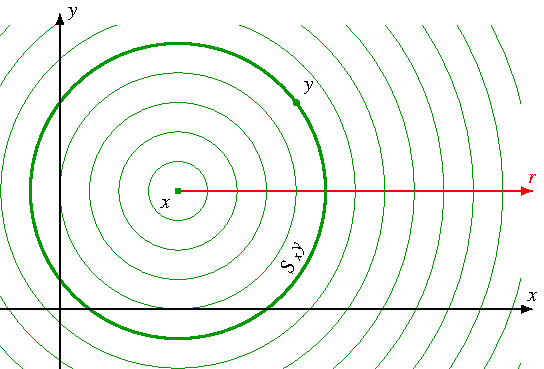
\includegraphics{chapters/070-nichtkomm/images/2dmendez.pdf}
\caption{Die Méndez-Transformation einer Funktion $f$ in der
Ebene an der Stelle $x,r$ ist der Mittelwert der Funktionswerte
auf auf dem Kreis $S_xy$ mit Radius $r=|y-x|$ um den Punkt $x$.
\label{buch:nichtkomm:mendez:fig:2d}}
\end{figure}
Für das Registrierungsproblem auf der Ebene mit der Gruppe
$\operatorname{SO}(2)\ltimes \mathbb{R}^2$ sind die Orbits des
Stabilisators eines Punktes $P=(x,y)$ Kreise vom Radius $r$ um
den Punkt (Abbildung~\ref{buch:nichtkomm:mendez:fig:2d}).
Der Raum $K\backslash G/K$ besteht aus den nichtnegativen
Zahlen $\mathbb{R}_{\ge 0}$.
Die Méndez-Transformation von $f$ hat daher die Werte
\[
\mathcal{M}f(P)(r)
=
\frac{1}{2\pi}
\int_0^{2\pi}
f(x+r\cos\varphi,y+r\sin\varphi)\,d\varphi.
\]
\end{beispiel}

\begin{beispiel}
\begin{figure}
\centering
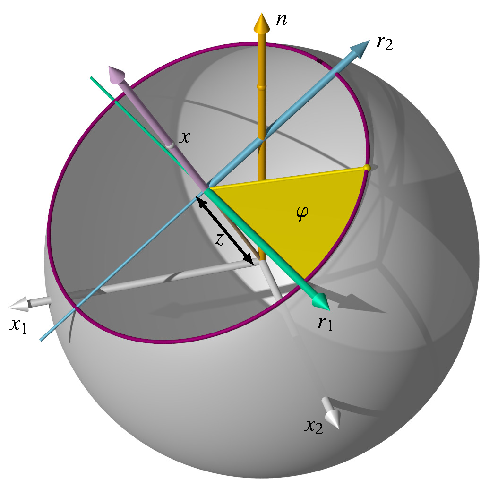
\includegraphics{chapters/070-nichtkomm/images/coordinates.pdf}
\caption{Koordinatensystem zur Berechnung der Méndez-Transformation
für das Paar $(G,K)=(\operatorname{SO}(3),\operatorname{SO}(2))$.
Die Koordinaten $z$ wird entlang der Achse mit Richtungsvektor $x\in S^2$
gemessen.
\label{buch:nichtkomm:mendez:fig:coordinates}}
\end{figure}
Für das Registrierungsproblem auf der Kugeloberfläche ist $x$ irgend ein
Einheitsvektor.
Die Orbits des Stabilisators von $x$ sind die Breitenkreise bezüglich
der Achse der Kugel durch $x$.
Sie sind durch die Höhe über der zu $x$ orthogonalen Äquatorebene der
Kugel charakterisiert.
Die Méndez-Transformierte einer Funktion $f\colon S^2\to \mathbb{R}$
an der Stelle $x$ ist daher eine Funktion $[-1,1]\to\mathbb{R}$ mit
dem Wert
\[
\mathcal{M}f (x)(z)
=
\int_{S_x} f(k\tilde{z})\,dk,
\]
wobei $\tilde{z}$ ein Einheitsektor mit $\tilde{z}\cdot x=z$ ist.
Das Integral ist der Mittelwert von $f$ über den Breitenkreis
auf Höhe $z$ um die Achse $x$.

In Abbildung~\ref{buch:nichtkomm:mendez:fig:coordinates} ist die
Achsrichtung $x\in S^2$ als hellvioletter Vektor eingezeichnet.
Die Koordinate $z\in[-1,1]$ wird vom Kugelmittelpunkt entlang dieser
Achse gemessen.
Zur Berechnung der Méndez-Transformation einer Funktion $f$ muss die
Funktion über den violett eingezeichneten Breitenkreis zur Achse $x$
integriert werden.
Dies kann mit Hilfe eines Integrals über den gelb eingezeichneten
Winkel $\varphi\in[0,2\pi]$ erfolgen.
Die Achsrichtungen $r_1=(n\times x)^0$ und $r_2=x\times r_1$ werden
aus der Richtung $n\in S^2$ des Nordpoles und $x$ berechnet.
Der Punkt mit Parameter $\varphi$ ist dann
\[
zx
+
\!\sqrt{1-z^2}(r_1 \cos\varphi + r_2 \sin\varphi).
\]
Die Méndez-Transformation kann damit als das Integral
\[
(\mathcal{M}f)(x)(z)
=
\frac{1}{2\pi}
\int_0^{2\pi}
f\left(
zx
+
\!\sqrt{1-z^2}(r_1 \cos\varphi + r_2 \sin\varphi)
\right)
d\varphi
\]
berechnet werden.
\end{beispiel}

Die Méndez-Transformation wurde von Tabea Méndez in 
\cite{buch:mendez} zur Lösung des Registrierungsproblems erfunden
und in \cite{buch:mendez-mueller} weiter verallgemeinert.
Die allgemeinste Darstellung der Theorie ist \cite[chapter 3]{buch:reg},
wo auch der Zusammenhang zur Radon-Transformation hergestellt wird.

%
% Lösung des Registrierungsproblems
%
\subsection{Lösung des Registrierungsproblems mit der Méndez-Transformation}
Es wurde bereits dargelegt, wie die Struktur des homogenen Raumes $G/K$
ermöglicht, das Registrierungsproblem in zwei einfachere Teilprobleme
zu zerlegen, nämlich das Finden eines Punktepaares, gefolgt von einem
Registrierungsproblem bezüglich der Gruppe $K$.
Mit der Méndez-Transformation kann der zweite Schritt jetzt vereinfacht
werden.
Wir zeigen hier nur das Prinzip, Optimierungsmöglichkeiten sind in
\cite{buch:mendez-mueller} und \cite{buch:reg} dargestellt.

%
% Registrierung mit einem Fixpunkt
%
\subsubsection{Registrierung mit einem Fixpunkt}
\begin{figure}
\centering
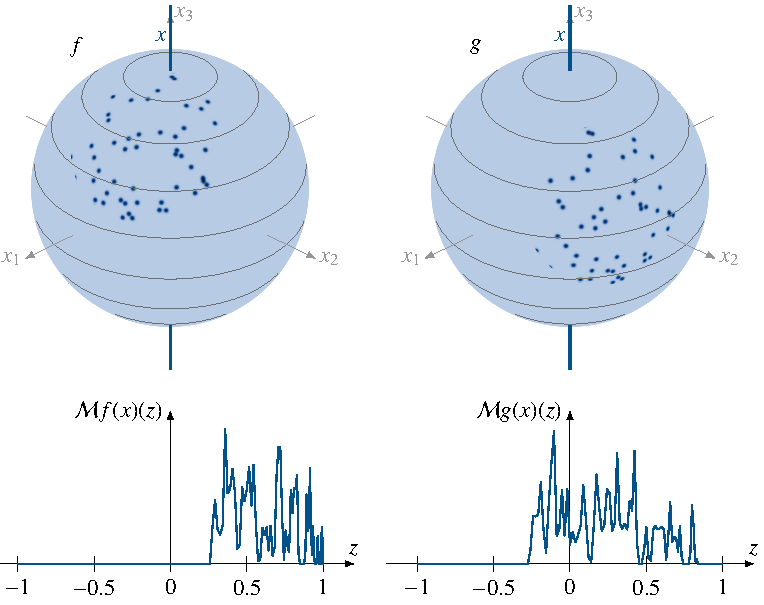
\includegraphics{chapters/070-nichtkomm/images/MTransformExamples.pdf}
\caption{Méndez-Transformation der zwei Funktionen $f$ und $g$ auf
der Kugeloberfläche.
Die $x_3$-Achse ist nicht die Drehachse der Drehung, die $f$ in $g$
überführt und die Méndez-Transformationen $\mathcal{M}f(x)$
und $\mathcal{M}g(x)$ sind klar verschieden.
\label{buch:nichtkomm:fig:mtex}}
\end{figure}
\begin{figure}
\centering
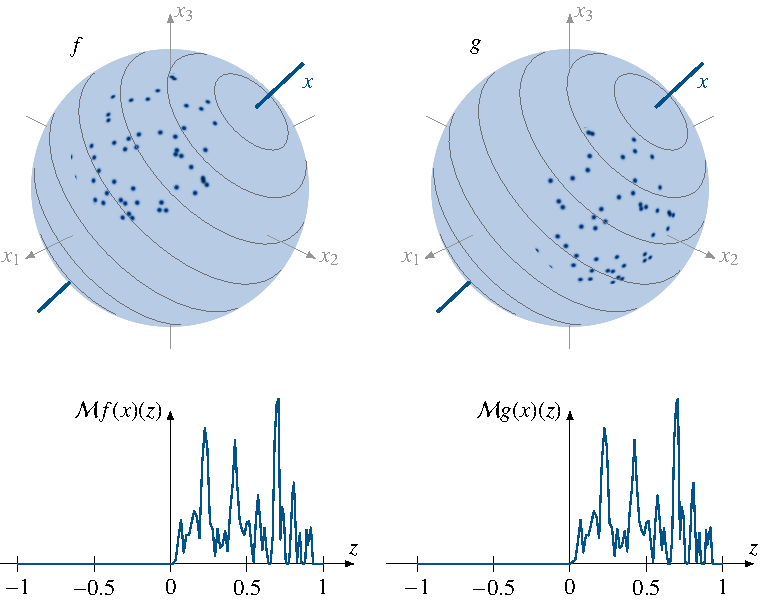
\includegraphics{chapters/070-nichtkomm/images/MTransformExamples2.pdf}
\caption{Méndez-Transformation der zwei Funktionen $f$ und $g$ auf
der Kugeloberfläche.
Die Achse mit Richtungsvektor $x$ gehört zu derjenigen Drehung,
die $f$ in $g$ überführt.
Die Méndez-Transformationen $\mathcal{M}f(x)$
und $\mathcal{M}g(x)$ sind gleich.
\label{buch:nichtkomm:fig:mtex2}}
\end{figure}
Falls die Wirkung der Gruppe $G$ auf $X$ immer einen Fixpunkt hat,
ist der erste Schritt des Registrierungsproblems besonders einfach
zu lösen.
In diesem Fall gibt es nämlich immer einen Punkt $x$, der beiden
Bildern gemeinsam ist.
Die Méndez-Transformationen $\mathcal{M}f(x)$ und $mathcal{M}g(x)$
sind daher die gleiche Funktion auf $Z=K\backslash G/K$.
Es muss daher nur der Definitionsbereich $X$ nach einem Punkt
durchsucht werden, für den $\mathcal{M}f(x) = \mathcal{M}g(x)$
gilt.
Da die Méndez-Transformation linear ist, bedeutet dies, dass nur
nach einer Nullstelle der Méndez-Transformation von $f-g$ gesucht
werden muss, also nach einem Punkt $x$, für den die Funktion
\(
\mathcal{M}(f-g)(x)
\)
die Nullfunktion ist.
Unter Berücksichtigung des Bildrauschens ist als $x$ so zu bestimmen,
dass die Norm $\| \mathcal{M}(f-g)(x) \|$ von $\mathcal{M}(f-g)(x)$
als Funktion auf $Z$ minimiert wird.

Das Registrierungsproblem auf der Kugeloberfläche gehört in diese
Klasse, den jede räumliche Drehung hat eine Drehachse, die fest
bleibt.
Das Finden eines Punktes mit $\mathcal{M}f(x)=\mathcal{M}g(x)$ 
kann immer noch eine ziemlich schwierige, nichtlineare Aufgabe sein.
Es ist aber nur noch ein zweidimensionales Problem, der Definitionsbereich
$S^2$ ist daher leichter zu durchsuchen als der dreidimensionale
Definitionsbereich $\operatorname{SO}(3)$.

Das Problem kann noch etwas vereinfacht werden durch die folgenden zwei
Beobachtungen, die in \cite{buch:mendez-mueller} etwas vertieft besprochen
werden.
\begin{enumerate}
\item
Für beliebige stetige Funktionen $f$ und $g$ ist die
Mendez-Transformation auch nur eine stetige Funktion und die
Abhängigkeit von $x$ ist im allgemeinen nicht differenzierbar.
Die Funktion $\|\mathcal{M}(f-g)(x)\|$ kann daher stark verrauscht
sein und es kann schwierig sein, das Minimum zu finden.
Durch Glättung der Funktionen kann erreicht werden, dass $f$ und $g$
differenzierbar sind, so dass das Minimum leichter zu finden ist.
\item
Glättung hat ausserdem den Vorteil, dass $x\mapsto\|\mathcal{M}(f-g)(x)\|_2^2$
eine differenzierbare Funktion ist, so dass ein gemäss 1.~gefundenes
approximatives Minimum mit Hilfe des quadratisch konvergenten Newtonschen
Algorithmus schnell verbessert werden kann.
\end{enumerate}

Weitere Möglichkeiten, die Lösung eines Registrierungsproblems mit
Hilfe eines Least-Squares-Ansatzes zu verbessern, sind in
\cite[chapter 3]{buch:reg} dargestellt.

%
% Registrierung ohne Fixpunkte
%
\subsubsection{Registrierung ohne Fixpunkte}
Beim Registrierungsproblem in der Ebene ist es möglich, dass die
Lösung ein reine Translation ist, die ausser im Fall der trivialen
Translation keine Fixpunkte hat.
In diesem Fall bleibt nichts anderes, als ein Punktepaar $x$ und $y$
zu finden so, dass $\mathcal{M}f(x)$ und $\mathcal{M}g(y)$ als Funktionen
auf $Z=K\backslash G/K$ übereinstimmen.
Dies sieht auf den ersten Blick nach einem sehr viel aufwendigeren
Problem aus, weil der Raum aller Punktepaare der vierdimensionale
Raum $\mathbb{R}^2\times\mathbb{R}^2$ ist.
Zwei Einschränkungen zeigen aber, dass dies nicht wirklich die
Schwierigkeit ist.
\begin{enumerate}
\item
Praktische Registrierungsprobleme suchen nur nach einer Translation
über eine beschränkte Distanz, gegeben durch die endliche Grösse 
der beiden Bilder.
\item
In einem realistischen Registrierungsproblem gibt es meistens einen
bekannten Bildpunkt des ersten Bildes, von dem man weiss, dass er auch
im zweiten Bild irgendwo vorkommt.
Es muss jetzt also nur noch der entsprechende Punkt im zweiten Bild
gesucht werden, was das Problem auf ein zweidimensionales Problem
reduziert.
\end{enumerate}




%%
% 6-registrierung.tex
%
% (c) 2022 Prof Dr Andreas Müller, OST Ostschweizer Fachhochschule
%
\section{Registrierung
\label{buch:nichtkomm:section:registrierung}}
\kopfrechts{Registrierung}


%\section*{Übungsaufgaben}
%\rhead{Übungsaufgaben}
%\aufgabetoplevel{chapters/010-potenzen/uebungsaufgaben}
%\begin{uebungsaufgaben}
%\uebungsaufgabe{101}
%\uebungsaufgabe{102}
%\uebungsaufgabe{103}
%\uebungsaufgabe{104}
%\end{uebungsaufgaben}

